\chapter{Theory}
\label{chap:theandme}
This chapter is divided into three parts. The first part introduces basic concepts of linguistics and natural language processing. Deep learning basics, with a focus of this work in mind, are presented in the second part. The third part of this chapter offers a more detailed explanation of methods directly relevant to this work (especially BERT model).

\section{Linguistics and \gls{nlp}}


%\subsection{Linguistics and Natural Language Processing -- Basic concepts}
Natural language processing can be described as a science at the border of linguistics and computer science although according to \citep{Wilks}, NLP itself is not a subject of a scientific research, it is rather a collection of problems, which can be examined. These tasks are drawn from general linguistics field and the goal is to solve (or \textit{process}) them by computers. General linguistics is a science which study and describes language. Its focus can be divided into following sub-fields: phonetics, phonology, morphology, syntax, semantics and pragmatics. 
This work is focused on task belonging into morphology (lemmatization, POS tagging) and semantics (sentiment analysis). More detailed description of tasks can be found in following subsections and in dedicated chapters for each task. Apart from tasks introduction, this chapter also includes a brief NLP history overview and a presentation of possible language data types.   %TODO odkazy? 


%Začít někde tady NLP věda na hranici lingvistiky a computer science
%a vysvetlit co patri do ligvistiky (co to je lingvistika) a co patri do comp science (+ def)
%Overlap between computer science and linguistics can be seen in natural language processing or computational linguistics. Although these two terms are often interchangeable, according to \citep{Wilks}, they are different. \citep{Wilks} states, that natural language processing by computers is called computational linguistics. 
%Natural language processing itself is not a subject of a scientific research, it is rather a collection of problems (like machine translation, summarization etc.), which can be examined. On the other hand, computational linguistics (CL) is a subject of research itself. Into problems connected with CL falls more technical ones -- part-of-speech tagging, syntax parsing, lemmatization -- which are not directly useful for non-expert users, but they can serve as a tool for proving linguistic theories or for achieving more sophisticated NLP tasks. %TODO nejaky zaver z tohoto odstavce? najit dalsi relevantni zdroje, co sem napsat dál? 

%TODO do záveru napsat, co bude v dalších podkapitolách


\subsection{Morphology}
Morphology studies an internal structures of words.
% todo do obrázku když už Basic building block of a word is a morpheme and such morphemes can represent semantics (meaning) or grammatical role of the world. %příklad
%One word can occur many forms created via inflection. %todo like apple - apples, 
%Such a set of all possible forms is called lexeme. Morphology is eldest lingusitical field % zdroj, 
%early automated models for morphological language processing focused on generating forms from lemmas % zdroj, Two level morphology
 % obrázek 
Morphology is used for many tasks, which can be divided into generative and analytical tasks. Generative tasks focuses on generation of word forms for given grammatical category. This can be useful for machine translation, full-text searching, labeling of documents by their key words or spell check. Result of a morphological analysis is a set of possible lemmas and tags for given word form. This set can be further narrowed by lemmatization (selection of the one "right" lemma), morphological tagging (selection of one right tag in given context), partitional disambiguation (removes all tags and lemmas, which can be reliably removed).

\par
\subsubsection{Lematization task}
Lemmatization task consist of finding a \textit{lemma}. Lemma is one chosen form of a word, selected to represent whole set of all possible word's forms (such set is called lexeme).  Which form is used as lemma is chosen by a convention -- for noun it is nominative of singular, for verb its infinitive etc.
\par
For example, lexeme for a czech word \textit{jablko} is \textit{jablko, jablka, jablku,  jablkem, jablek, jablky, jablkům} and lemma is \textit{jablko}.

\subsubsection{Part-of-speech tagging} 
Part-of-speech tagging classifies word into one of part-of-speech categories (like noun, pronoun, verb, etc) \citep{Hladka}. Part of tagging can also be a determination of grammatical categories (like case, number, tense). %TODO obrázek s príkladem 
Czech morphology developement is dated from 1989 %TODO zdroj Hajič.
and in description of words uses 15-places morphological tags \citep{Hana2005}.
A more detailed description of each position can be seen in table \ref{Tab:tagset}.

\begin{table}
\centering
\label{Tab:tagset}
\begin{tabular}{ |c|c|c| } 


 \hline
 Position & Name & Description \\ 
 \hline \hline
 1 & POS & Part of speech \\ \hline
 2 & SubPOS & Detailed part of speech \\ \hline
  3 & Gender & Gender \\ \hline
4 & Number & Number \\\hline
  5 & Case & Case \\ \hline
 6 & PossGender & Possessor's gender \\\hline
  7 & PossNumber & Possessor's number \\ \hline
8 & Person & Person \\\hline
  9 & Tense & Tense \\ \hline
 10 & Grade & Degree of comparison\\\hline
  11 & Negation & Negation \\ \hline
 12 & Voice & Voice \\\hline
 13 & Reserve1 & Reserve \\ \hline
14 & Reserve2 & Reserve \\\hline
  15 & Var & Variant, style \\ 
 \hline

\end{tabular}
\caption{Table from \citep{Hana2005} describes all 15 positions of Czech morphological tagging.
} 
\end{table}


\subsection{Semantics}
Semantics is dealing with word meaning. This is definitely more complicated object of study even for humans, let alone for computers. Word meaning can be subjective, change during historical periods, sentence is not simple sum of meanings of its words and many other problems comes with efforts of learning computers to truly understand a human language.

Sentiment analysis can be useful for various tasks from natural language text generation to recognition of homonymy or polysemy of given words. It could solve sophisticated assignments as answering questions about the input text document or help in high-quality translation. Another possible task is to find in the text so-called named entities - like persons, months or cites - or linking these entities to some knowledge base. 
\subsubsection{Sentiment analysis}
An input of a sentiment analysis is a text and the output is a classification into one of categories. In this work, categories are positive, negative and in some data sets also neutral, but it is also common to use labels like abusive or ironic.
As a part of sentiment analysis can be involved so-called subjectivity\citep{Montoyo2012}. The goal of subjectivity prediction is to classify if the
opinion (both positive or negative) is objective or the author is personally interested and has strong emotions about his claims. For example, the following text could be recognized as objective: “The sound of this notebook is clear.”, “The base is not stable enough.” or even “An internet connection in this area is bad.” in contrast with “I hate the way the new touchpad works.”. The subjectivity of the claim does not depend on its sentiment. This part of sentiment analysis was not included in this work and it is mentioned just for completeness. %TODO

\subsection{Language data}
Inputs to natural language processing can be formed by data of many kinds and can be categorized by a form or by a source. 
As for form, we can work with corporas or datasets of various sizes, containig data from many sources. A corpora is a large collection of texts, which aims to be in some way representative sample of a language. This is not fully possible, mainly because the selection of examples in the corpus is limited compared to a diversity of language. Most famous linguistic corporas are co-called Brown corpus \citep{francis79browncorpus} -- first electronical corpora mixed from newspaper articles and beletry, and PennTreebank \citep{Marcus1993}, which si first syntactically anotated corpus, but has quite domain limited source - articles from Wall Street Journal. One of corpora's type is a treebanks. A treebank is a parsed corpus with various types of annotations and uses trees for representation of dependencies. An example of such trees can be seen on figure \ref{fig:trees} and an example of a treebank is presented on picture \ref{fig:treebank}
%TODO - kouknout do poznámek.
The question arises as to what is the difference between a corpora and a "simple" dataset. Sometimes these terms can be interchangeable in the sense that the usage of both can be the same. In some cases, both types of data can be used for the same task, but the difference is more theoretical. The idea of a corpora is to collect somehow representative sample of a language with annotations on many levels which allows a performation of different analysis upon this data. Dataset is typically created on restricted domain (like tweets on US Airlines pages \footnote{https://www.kaggle.com/crowdflower/twitter-airline-sentiment} or movie reviews \footnote{https://www.kaggle.com/lakshmi25npathi/imdb-dataset-of-50k-movie-reviews}) 
and are annotated for one type of task (in this case sentiment).  
\begin{figure}[h]
\centering
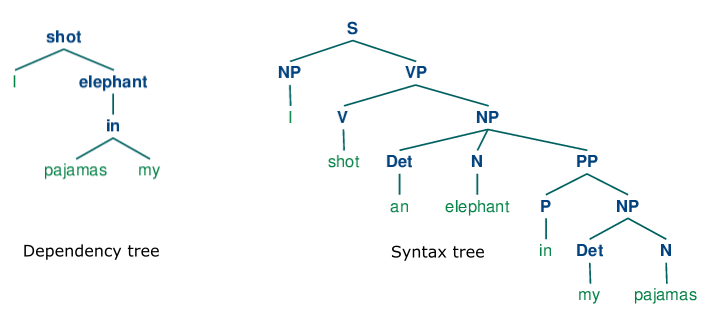
\includegraphics[width=1\textwidth]{../img/syntax_depedency_trees.png}
\caption{
An example of the syntax and dependency tree. Dependency tree, as the name indicates, describes dependencies between words. Such dependencies are of various types, for example an elephant in the example is an direct object of the shooting action. A root of such tree is typically a predicate of the sentence. On the other hand, syntax tree represents syntactic structure of the sentence according to the grammar. The root of the tree is \textit{sentence}, which is split to noun and verb phrase. These can be further divided into phrases compound from particular instances of parts of speech (e.g. nouns, adverbs, verbs, prepositions etc).
\newline \textit{Source: \cite{NLTKbook}}}
\label{fig:trees}
\end{figure}

\begin{figure}
\centering
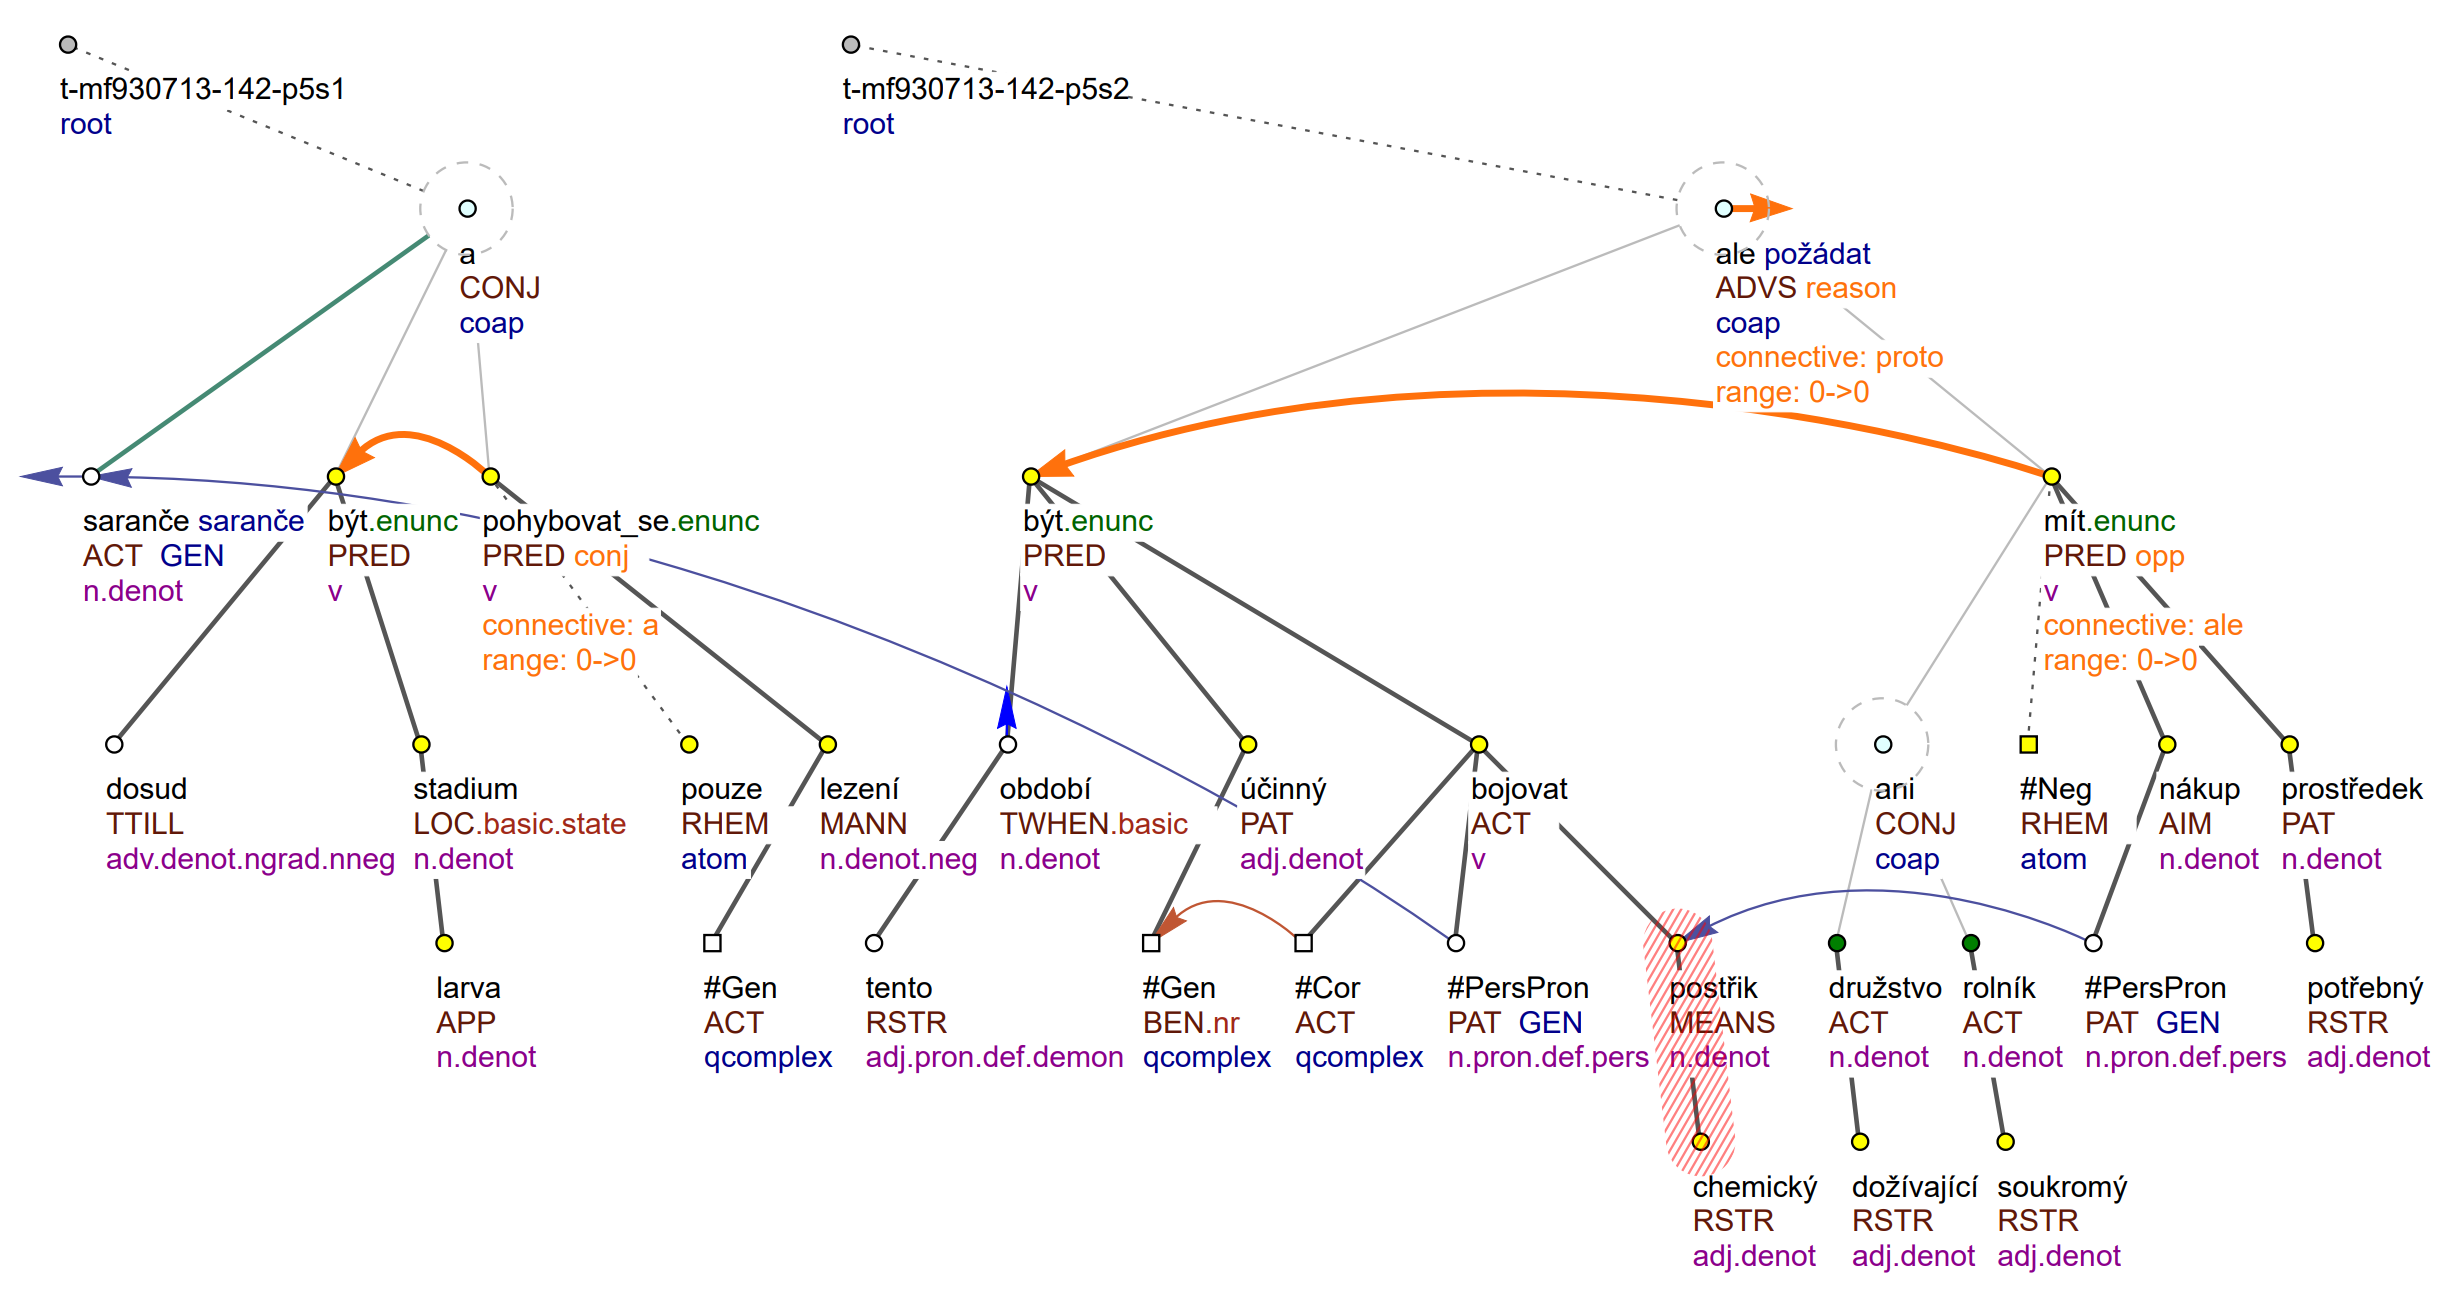
\includegraphics[width=1\textwidth]{../img/prague_dep_treebank.png}
\caption{
Prague dependency treebank example \cite{PDT35} for the sentences:
\textit{Grasshoppers are still in the larvae stadium, crawling only. At this time of the year, it is efficient to fight them using chemicals, but neither the ailing cooperatives nor private farmers can afford them.} czech: \textit{Sarančata jsou doposud ve stadiu larev a pohybují se pouze lezením. V tomto období je účinné bojovat proti nim chemickými postřiky, ale dožívající družstva ani soukromí rolníci nemají na jejich nákup potřebné prostředky}. This treebank contains dependency trees, but is is just one of many possibilities. This example is from Prague dependency treebank, which offers different layers of annotations. Red strips over words \textit{chemický} and \textit{postřik} marks multiword phrase, conjunction between \textit{rolník} and \textit{družstvo} is expressed as by one type of nodes, blue lines denotes coreference etc.} Praque dependency treebank data are used for tagging and lemmatization tasks.
\label{fig:pdt}
\end{figure}

Data in both dataset and corpora can come from many written or oral sources. For machine translation documents with many language versions are appropriate. An example of the use of such multilingual documents is a project Eurotra \citep{oakley1995final}.
Eurotra was almost twenty years lasting project of the European Commission dedicated to machine translation started on the latest seventieths. EU administrative documents in French and English served as datasets. %TODO jak byli kvalitní
Linguistic data can differ in quality and a length.  Relatively new source of data are social networks like twitter, reddit or facebook. Data from some social networks (facebook, twitter) are very different from more traditional sources like scientific papers, newspaper articles or books.  These data are short snippets of text full of odd characters, newlines, and ends of lines. They contain pictures, emoji, a mixture of different languages, slang expressions, and grammatical errors. And they are very short, sometimes they consists only of one sentence, few hashtags and a link or a picture. Because people share their opinions, emotions and are ready to do their choices according to incoming influences, social networks are very important source of information. Big problem while analysing this data is their amount. Only a twitter uses produce about 12 TB of data per day \footnote{https://bigdatashowcase.com/how-much-big-data-companies-make-on-internet/}. it is not possible to process all the data manualy so this is one of reasons for importance of natural language processing.  %TODO nemá to být v úvodu?

\subsection{Historical Development}
Historical development of computer linguistics was significantly affected by machine translation \citep{Wilks}. Many important milestones in the history of machine translation also improved other parts of \gls{nlp}, so I will briefly present its historical development. First attempts to translation started in 1933 by patents for machine translations (mechanical multilingual dictionaries) \citep{Hutchins}
followed by a big boom of machine translation in the 50s and 60s and than continued by a slowdown after ALPAC report in 1966 \citep{Hutchins1996}. 

First attempts to machine translation were based on bilingual dictionaries and sets of rules. Such translation was based on a translation of individual word or a group of words with a subsequent improvement of syntax and morphology. Resulting translation weren't good and required lots of work of human work of expert linguists. This approach was replaced around year 1990 by a statistical translation \citep{Brown}. Central idea of a statistical machine translation is a probability of a translated sentence, given the original sentence. This includes also a probability of resulting sentence in the target language. Such probabilities were computed using frequencies of words or their sequences (n-grams) in large language corpus. \citep{jurafsky2012natural} %TODO nejake vysledky, SOTA? 
These methods were quite successful but they suffered from the curse of dimensionality \citep[p.450]{Goodfellow-et-al-2016}.  %TODO str 450 z DLbook
Next stage of machine translation (and also other NLP tasks) starts with the second wave of a popularity of neural networks.
There is too many possible words or n-grams of words and there is no way how to share learned informations between similar words or sequences in statistical methods. A solution of this problem can be seen in the paper \citep{Bengio2003}, where authors presented neural trained word embeddings (see \ref{sec:embedd}). Even better results were obtained by neural language models (probabilites of words are learned by neural network) \citep{Schwenk2006}. Current natural language processing is built on deep recurrent neural networks and encoder-decoder architecture, firstly published in \citep{Cho2014}, \citep{Sutskever2014} and \citep{Wu2016}.

In current times, not only machine translation systems but any other linguistic tasks are solved by neural networks. State-of-the-art result for machine translation, sentiment analysis and many others hold by methods based on depp learning \footnote{http://nlpprogress.com/}. For that reason, the following subsection presents deep learning basics, their usage and improvements in \gls{nlp} in recent years.

\section{Deep Learning}
Neural networks are designed as supervised machine learning techniques. It means that input data consist of two-part examples -- observations and correct response for each observation. Supervised methods than tries to produce an output which will correctly predict responses. \citep{Russell1995}
\par
Supervised machine learning problems can be distinguished by the desired outcome as classification or regression. Classification means that we want to sort data into one of predefined classes, meanwhile regression's gaol is a numerical result. In the case of multi-class classification, true results (labels) can be in one of following forms --  text, numbers or one-hot vector. If there are more than two classes presented, one-hot vector has length equal to number of classes and consist of zeros on every indices but target class index, where is one.
 %TODO sjednotit label, response, 

\subsection{True ML Goal and Regularization}
Supervised machine learning goal is not to predict correctly all labels in example data, but to predict correctly all possible inputs from the distribution example data are taken from. During training there can appear a problem called \textit{overfitting}. As showed in Figure \ref{pic:overfitting}, 

\begin{figure}[h]
\centering
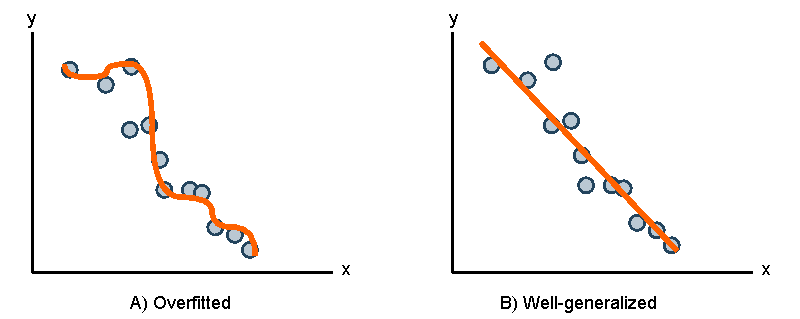
\includegraphics[width=0.7\columnwidth]{../img/overfitting}
\caption{Figure A) presents overfitting scenario. Figure B) illustrates possible well-generalized solution. }
\label{pic:overfitting}
\end{figure}
overfitting problem is that result prediction function practically memorized all training data examples and can minimize the error on them very nicely, but probably will not perform well on previously unseen data. Regularization is a tool for preventing such issues. Well known regularization techniques like lasso regression \citep{Tibshirani1996} or ridge regression \citep{Hoerl1970}, which are used for linear regression, works by adding some new members into the sum for the loss function which should be minimize. %TODO english improvement
Another classification regularization method, which is also used in this work, is label smoothing.
\par
Label smoothing \citep{Szegedy2015} is an idea applicable to every classification problem, therefore is not limited to a NLP only.
In any classification task, training data contains labels of the correct classes. In binary classification or one-hot encoded labels, correct class is denoted by 1 and incorrect class(es) by 0. Instead of this, label smoothing applies following formula: 
$$y_{new} = (1 - \epsilon) * y + \alpha / K$$, where $K$ is number of classes. Label smoothing is used as a cure for overfitting and overconfidence in the case of use of a softmax 
 as output activation function. Loss function for softmax classification is: 
 $$ loss = -\sum_{i=1}^{n} \sum_{y=1}^{K} p(y \mid x_i) log \, q_{\theta} ( y_i \mid x_i ) $$
 and after substitution of label smoothing\footnote{Taken from: https://leimao.github.io/blog/Label-Smoothing/}:
$$
loss_{ls} = -\sum_{i=1}^{n} \sum_{y=1}^{K} [(1-\epsilon) p(y \mid x_i)+\epsilon u(y\mid x_i)]log \, q_\theta(y \mid x_i) $$,
which gaves after multiplication\footnote{Taken from: https://leimao.github.io/blog/Label-Smoothing/}:

 \begin{equation} \label{eq:lsloss}
 loss_{ls}= \sum_{i=1}^{n} {(1- \epsilon)[- \sum_{y=1}^{K} p(y\mid x_i) log \, q\theta(y \mid x_i)]+\epsilon [- \sum_{y=1}^{K} u(y \mid x_i)log \, q\theta (y\mid x_i)]}
 \end{equation}

From equation \ref{eq:lsloss} can be seen, than if the network is very confidential about some prediction, second part of loss function is very large, so label smoothing works as a regularization of overconfidence.

\subsection{Deep Learning History}
The history of learning algorithms inspired by a human brain started in the 1940s under the name \textit{cybernetics} \citep{Goodfellow-et-al-2016}, \citep{McCulloch}. First such architecture was a perceptron \citep{Rosenblatt1958}.
Perceptron , found in 1958, is the simplest neural network with just one layer serving for binary classification (see Fig. \ref{pic:perceptron}). Input of a perceptron is a vector of features describing an input example and an output is classification into class 0 or 1.

\begin{figure}[h]
\centering
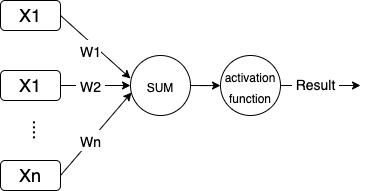
\includegraphics[width=0.8\columnwidth]{../img/perceptron}
\caption{A one-layer perceptron architecture. The result is formed by the application of activation function on a weighted sum of inputs. Weights are updated during training till it returns satisfactory results. }
\label{pic:perceptron}
\end{figure}
There also exists a multi-class version for the general classification. The problem of this perceptron was the inability to classify data that are not linearly separable \citep{Minsky2017} (see Fig. \ref{pic:xor}), which led to a lack of interest in deep networks for some period.
\begin{figure}[h]
\centering
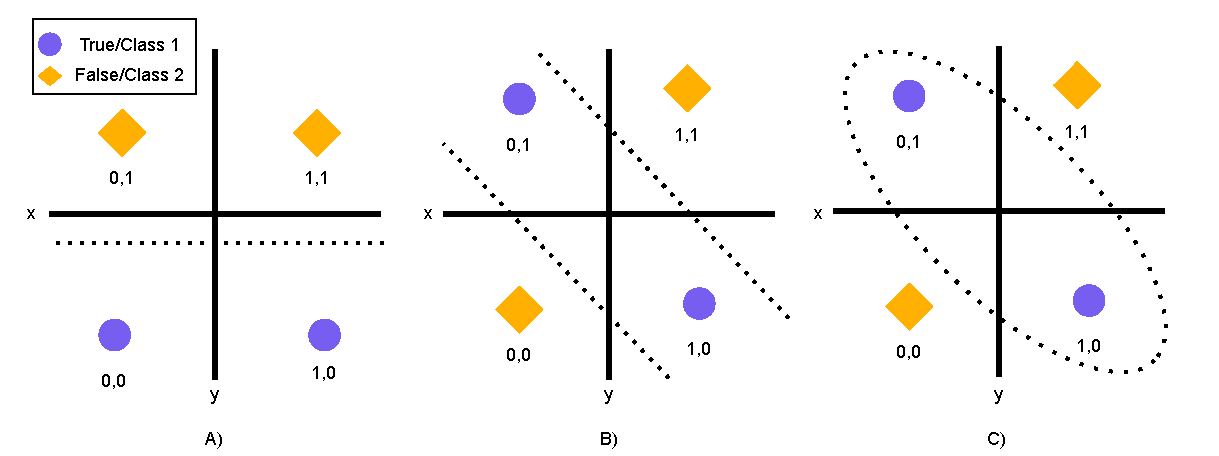
\includegraphics[width=0.6\columnwidth]{../img/xor}
\caption{This picture illustrates XOR problem. Perception can find the correct solution only if the data are linearly separable. It means, that they can be divided by a hyperplane. An example of such two-dimensional data can be seen in picture A). The dotted line shows a possible border for separation. Picture B) shows XOR problem. XOR is a logical operation on two boolean variables, which returns true if one variable is True (1) and the other one is False (0), and returns False otherwise. Such data cannot be separated by one hyperplane. Linearly non-separable data can be for example separated by a circle (pic. C)}
\label{pic:xor}
\end{figure}

Era of \textit{deep} neural networks started around year 2007 %TODO zdroj
with bigger datasets and greater computational resources. These two new features opened the possibility of neural network learning without expertly handcrafted parameters tuning with good results.
Many ideas which are currently frequently used are quite old - like backpropagation \citep{Rumelhart} or even encoder-decoder architecture \citep{Allen19}, \citep{Forcada1997}.

\par
The basic type of DNN is a multilayer perceptron (see picture \ref{pic:multilayer}).
It is combined with neurons, every neuron has an \textit{activation function} %TODO napsat něco
, which is applied to its input. Input to every, but the first layer is a weighted combination of (possibly selection of) previous layer neurons. 
Different types of NN differs by number and shape of layers, activation functions and connections between neurons. (see Fig. \ref{pic:multilayer}).
\begin{figure}[h]
\centering
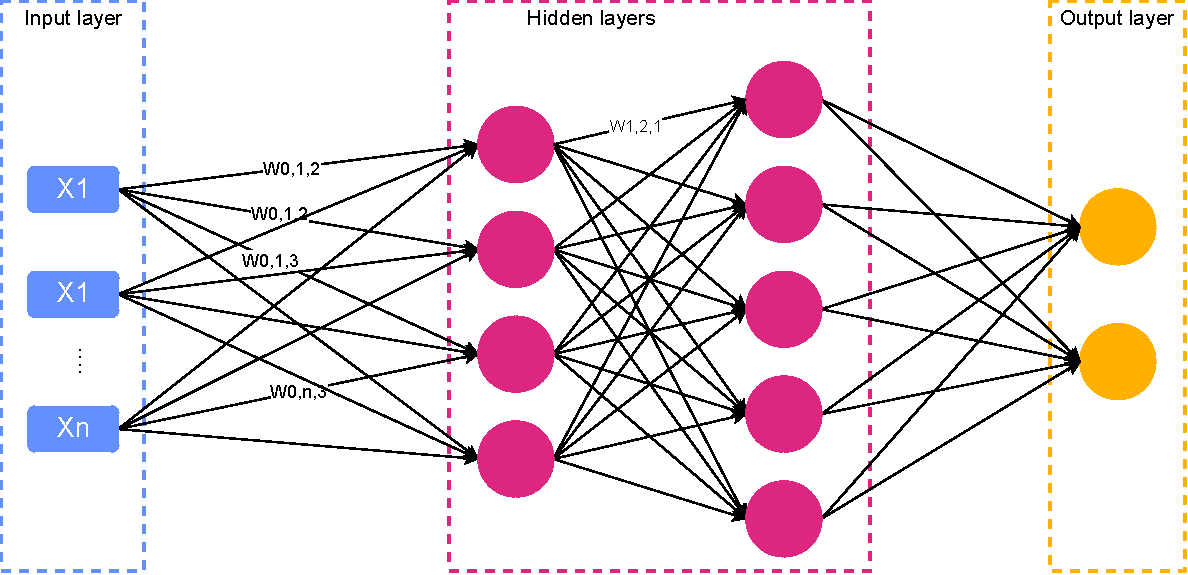
\includegraphics[width=1\columnwidth]{../img/multilayer}
\caption{Multilayer perceptron (or feed-forward neural network) is formed input and outpu layer and variable number of hidden layers with different sizes. In every layer, chosen application function is applied to a weighted sum of inputs from previous layer.}
\label{pic:multilayer}
\end{figure}

\par
Some of the key ideas for (not only) NLP and specifically for BERT, are presented in the following subsections.

\par
In NLP, same as in other machine learning methods, is necessary to decide how to encode the input to make it processable by computers and especially which input features are important for given task and should be included. These questions are in NLP addressed, among others, by two techniques: word embeddings (see section \ref{sec:embedd}) and attention mechanism (see section \ref{sub:attention}). Word embeddings deals with representation of words and their meaning, while attention mechanism determines which parts of text are relevant for given task.

Many machine learning methods are applied to data with no defined order between samples -- like a bunch of images or description of petals for each sample flower. %TDO odkaz
Language data are, however, different, because their nature is sequential. Word and sentences ordering is an important part of text and lack of it can make text absolutely nonsense. This problems can be more or less satisfactorily handled by Recurrent Neural Networks (in section \ref{sub:RNN}) and Transformers architecture (section \ref{sub:transformers}). Combination of all these methods led to a BERT models family, which are used for this work (see section \ref{sec:bert}).


\subsection{Embeddings}
\label{sec:embedd}
Good performance of NLP models relies on a text representation. What is hypothetically deserved is to teaching computers to understand semantics of language. Once computer has a good representation of what given text \textit{means}, it should be easy to answer questions, translate it into an another language etc. Because NN are able to work only with numerical representation of inputs, second requirement upon such language representation is to be numerical. Straightforward way is to represent input words in one-hot encoding. In one-hot representation single word is represented by a vector, where is only 1 at the position of respective word and all other positions are zeros. Such vector is long as a number of distinct words in a dictionary, so it could be quite large. Most important problem of one-hot representation is that every two words similarly distant to each other. It can be an advantage in some areas, but it is not true in linguistics. Words can have similar meanings or be opposite to each other, generally spoken a distance between them is not uniform.
\par
When compared to one-hot encoding, embeddings  \citep{Bengio2003}, \citep{Ling} are better solution for language data. Embedding is also a vector, which represent input word, but in contrast to one-hot encoding, its size does not depend on the vocabulary size. These embedding are not hand crafted by humans, they are learned by NN. They can be learned for every specific task from scratch or it is possible to use embeddings trained for usage in many tasks like in the following cases.
Before contextualized embeddings appeared, pretrained embeddings were created mainly by Word2Vec \citep{Mikolov2013}  
%TODO turian, mikolov, pennington -- embeddings normal
, specifically by its two variants: CBOW and SkipGram model.
CBOW model's objective is to predict a masked word from its context and SkipGram does exactly the opposite - predicting context of a given word. %TODO obrázek?
These predicting objectives serves just as a tool for forcing a network to learn useful word representation.  Embeddings are then imputed into network as a embedding layer at the beginning of the network with size $number\_of\_words \times embedding\_size$. We still need to bridge the gap between text and numbers, so it is possoble to use one-hot encoding or simple word numbering as an input into this first embedding layer.  Word2Vec-like embeddings uses just few context words and they does not use explicitly information about statistics in whole dataset. GloVe \citep{Pennington} embeddings, on the other hand, uses information about frequencies of pairs of words in a whole dataset and are designed to project word vectors into meaningful vector space. 
\\
Embeddings of previously described types though uses context of the word -- it is in fact how they are meant to work. Similar words are supposed to appear frequently in similar context. Problem of such embeddings is that an input word embedding in the first layer of neural network is computed independently on neighbour words, so the same word has always the same embedding regardless of the context. In the case of homonyms,non-contextualized embeddings are a mixture of all the (possibly very different) meanings, which can lead to poor results.  The problem with same word embedding in different context is definitely a problem in the case of homonyms, but also in other cases contextualized embeddings seems to give better results \citep{Straka2019a}, \citep{Liu2020}.

\subsubsection{Contextualized embeddings}
To solve the problem of different word meanings, contextualized embeddings where invented in recent years, namely BERT \citep{Devlin2019}, ELMo \citep{Peters2018} and XLNet \citep{Yang2019}. %TODO precist \citep{Raffel2019}.  - není nový typ, spíš souhrn
Contextualized embedding of a word is computed with a knowledge of the whole sentence dynamically for each word occurrence.
In addition to BERT, there are also other contextualized embedding architextures, namely GTP-2 %TODO zdroj radfford, 
and ELMo. Their comparison can be found in a subsection \ref{sub:specialBert}. 
%TODO pridat moznosti jak zapojit embeddings - dát k trénování a modelům
%TODO catastrophic forgetting
\par
As embeddings are trained after the input is encoded into one-hot vectors, it is impossible to use pretrained embedding for encoding of previously unseen words. This is solved by embeddings of characters or subwords, so the whole word embedding can be later compound of them. The possibilities of involving and training such embeddings are described in more detail in section \ref{sub:models}.

Embeddings are currently best option of input representation, but other part of problem is how to recognize, which parts of input are useful for given task. This problem is addressed by attention mechanism, described in the following subsection. 

\subsection{Attention mechanism}
\label{sub:attention}
Attention mechanism \citep{Bahdanau} is widely used in NLP as a tool for extracting relevant informations from word sequences. For example when generating translation of some sentence, each word in target language corresponds to just few words in source sentence, not to a whole sentence. Attention gives weights to the words, which represents this connections (see picture \ref{pic:att_trans}).

\begin{figure}[h]
\label{pic:att_trans}
\centering
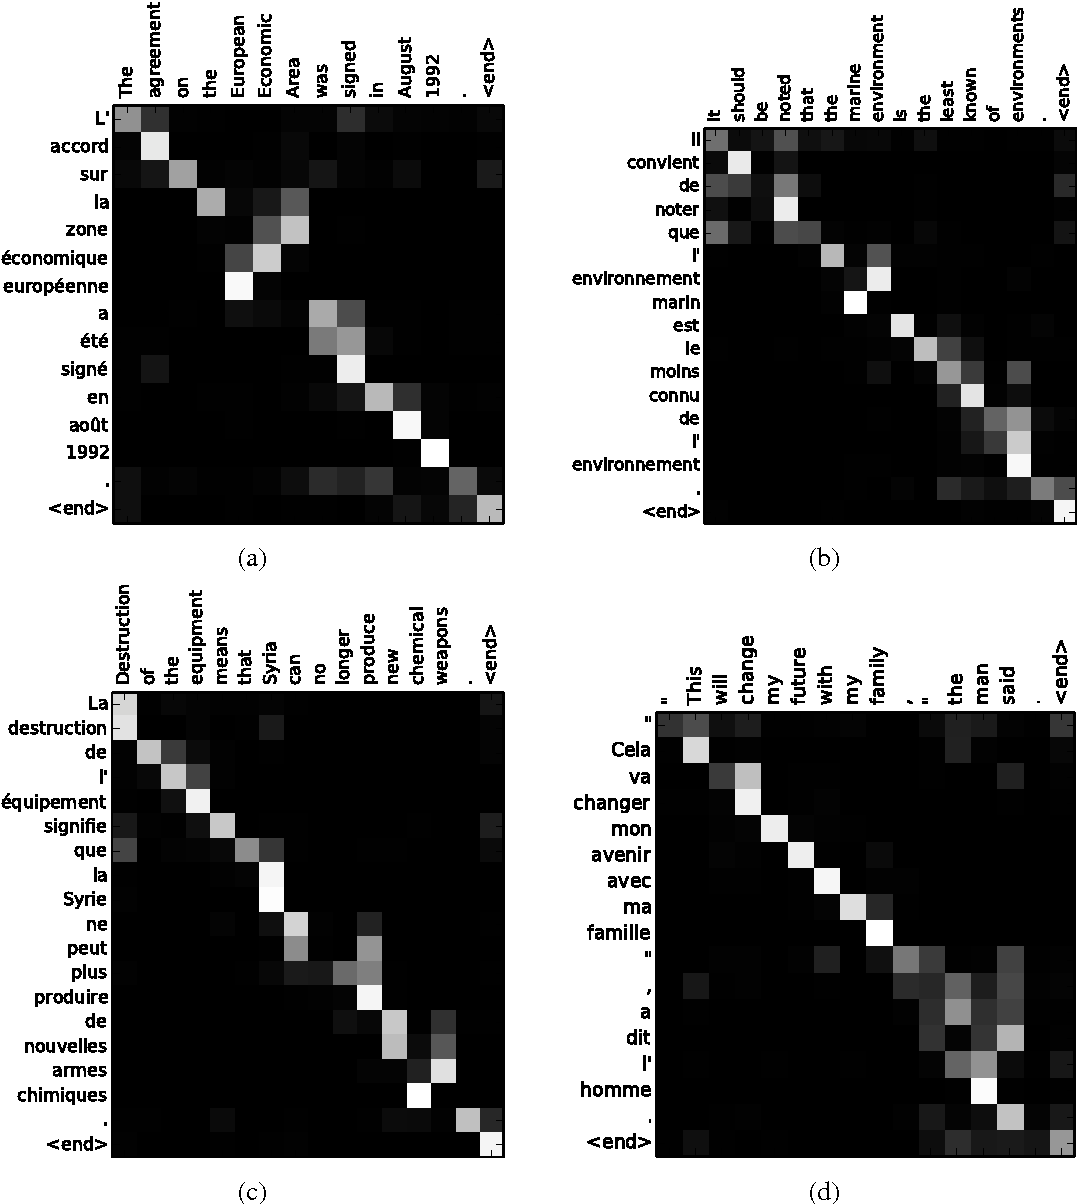
\includegraphics[width=0.7\columnwidth]{../img/attention_translate}
\caption{Figure 3 of \citep{Bahdanau}
}
\end{figure}


When the task is a question answering, attention can help a model to focus on relevant part in the text, where the answer is located \citep{Santos2016}. For example see picture \ref{pic:att_cnn}

\begin{figure}[h]
\label{pic:att_cnn}
\centering
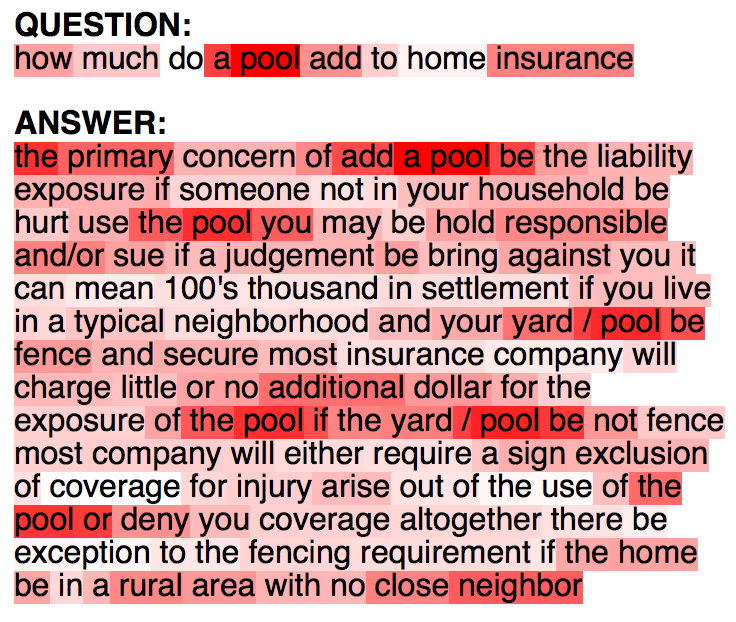
\includegraphics[width=0.7\columnwidth]{../img/attention_cnn}
\caption{Figure 3 of \citep{Santos2016}
}
\end{figure}
Same idea can be (and really is) applied into computer vision, where it imitates human behaviour. Humans also focuses on (or \textit{attend to}) just  a few parts of their visual input when they are, for example, recognizing things on pictures.
Modification to an attention concept, called self-attention \citep{Cheng}, deals with relationships inside one part of text (e.g. a sentence). This variant of attention do not connect one part of text (like question) to other different part of text (like answer), but only models relationships inside one part. Attention has three inputs -- key, value and query, all vectors. The output is weighted sum of values and the weights are computed with respect to key-query pair \footnote{This video series helped me a lot with an understanding of self-attention concept: https://youtube.com/playlist?list=PL75e0qA87dlG-za8eLI6t0\_Pbxafk-cxb}. For more explanation, see picture \ref{pic:att_self}
\begin{figure}[h]
\label{pic:att_self}
\centering
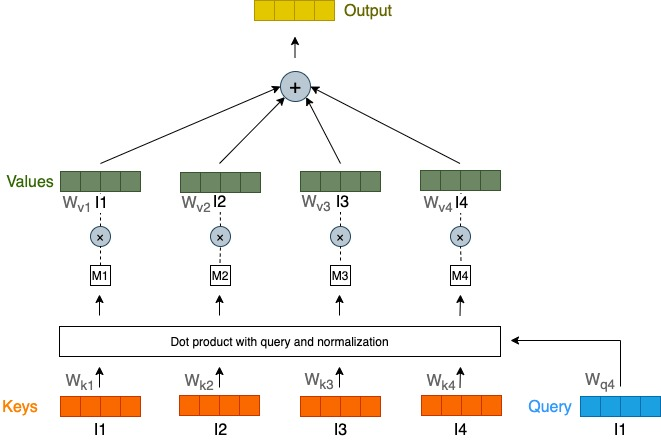
\includegraphics[width=1\columnwidth]{../img/self_attention1}
\caption{Self-attention mechanism scheme for one concrete query vector. The result is an embedding, which is improved by the context of the word. This picture illustrates result for first word embedding (l1) in a 4 words long text. Keys, values and a query are all multiplied by their respective weights ($W_k$, $W_v$ and $W_q$) before any other operation with them. These weights are trained during learning. Dot products between every word and a query are computed. Result is a number for every input word, so 4 numbers at the end. These numbers are normalized, so the sum of them is equal to 1. After that, these words serve as a weights ($M_x$), which indicates relationship between query and every other word. Resulting better embedding for the query is than obtained as a sum of the word embeddings weighted by these obtained weights. 
}
\end{figure}

\par
Together with transformers architecture, which is an important part of BERT and other language models used in this work, was also published a new approach to self-attention - \textit{multihead attention} \citep{Vaswani2017}. Multihead attention also tries to model relationships between the words in the same sequence. As it is multihead, it can, for one word, pay attention to more words (or their parts).  

\subsection{Language modelling}
\label{sub:models}
Contextualization of embeddings is not important only because it solves the problem of same words with different meaning, but also because they are supposed to store a knowledge independent on any language. %TODO proč? : (Liu et al., 2019a; Hewitt and Liang, 2019; Hewitt and Manning, 2019; Tenney et al., 2019a) demonstrate across languages

Contextualized embeddings can be obtained by supervised or unsupervised learning \citep{Liu2020}. This work focuses on unsupervised learning, as it is currently very promising field according to recent results and also because unsupervised learning does not depend on large manually created datasets. Supervised methods uses machine translation, which is the classic NLP task, but also natural language inference or other tasks with potential to capture general knowledge about language.

Unsupervised learning tries to learn a language model -- probability distribution over a sequence of tokens given by following equation:
 \begin{equation*}
  p(t_1, t_2,...,t_N) =\prod_{i=1}^{N} p(t_i | t_1, t_2, ..., t_{i-1})
\end{equation*}.



%%%%%%%%%%%%%%%%%%%%%%%%%%%%%%%%%GRU, LSTM, Transformers
\subsection{Recurrent Neural Networks}
\label{sub:RNN}
 %TODO napojit nějak normálně 
 % %TODO vysvetlit
Text sequences can be very long and related words often has logn distance in between. This places hard demands on neural networks, because such data structure differs from most of other NN applications, where input samples are independent and ordering does not matter. This can also leads to vanishing/exploding gradients, because information should be carried for many steps, which leads in many multiplications of very small or big numbers in neural networks.

The construction of such networks, which are able to capture natural language structure requires solving two problems:
\begin{itemize}
\item input should be understood by network as a sequence,
\item there must be a possibility to use information from other parts of sentence (and do not forget them).
\end{itemize}
 First problem was solved by simple Recurrent Neural Networks (RNN). To represent an ordering and a continuity of input words, basic RNN adds a connection between output for one word and an input for the next word (see picture \ref{pic:rnn}). 
 
\begin{figure}[h]
\centering
\includegraphics[width=1\columnwidth]{../img/rnn}
\protect\caption{Basic Recurent neural network architecture. It is composed by one rnn cell which recurrently uses informations from previous seen input. For better illustration of working in the time, RNN can be visualised as a chain of cells connected by a result of previous cell. source: \textit{Picture from https://medium.com/deeplearningbrasilia/deep-learning-recurrent-neural-networks-f9482a24d010}.}
\label{pic:rnn}
\end{figure}
 
 
 
The latter problem needs a more complicated approach. There are basically three attempts to solve this \textit{short memory} of RNN cells -- Gated Recurrent Unit (GRU) \citep{Cho2014}, Long Short Term Memory (LSTM) \citep{Hochreiter1997} and Transformers architecture \citep{Vaswani2017} with attention mechanism.
\par
Both LSTM and GRU uses an idea of gating. Term \textit{gate} refers to a weight (multiplication factor) for previous informations and new input. Gate determines which information from previous words should be remembered and which should be forgotten. To achieve this, gate is formed by sigmoid activation function, which range is from 0 to 1 and present a portion of remembered information. Previous informations are encoded in a cell state and a hidden state, both passed from cell to cell (with application of gates). Comparison of both architectures can be found on figure \ref{pic:lstm_gru}.

\begin{figure}[h]
\centering
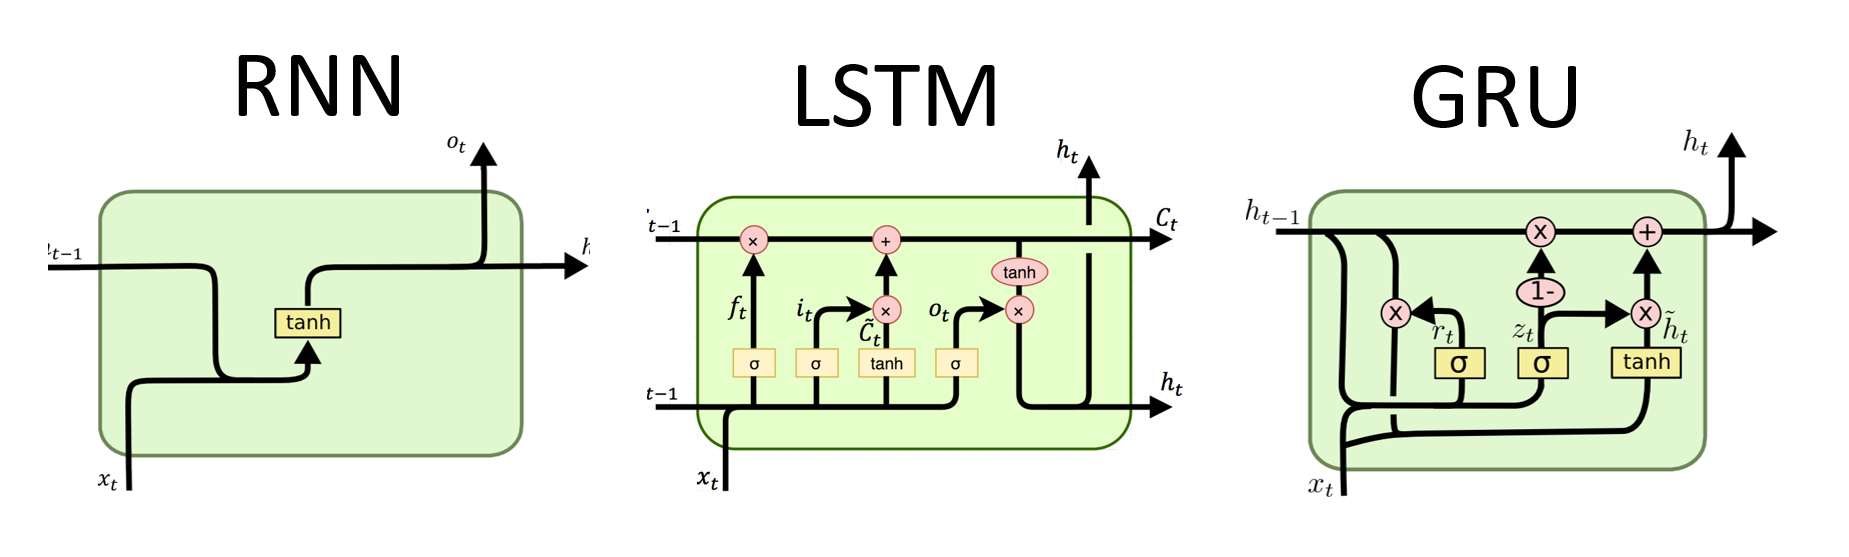
\includegraphics[width=1\columnwidth]{../img/lstm_gru}
\protect\caption{Comparison of LSTM and GRU architecture \textit{http://dprogrammer.org/rnn-lstm-gru}.}
\label{pic:lstm_gru}
\end{figure}
\subsubsection*{LSTM} LSTM cell uses input, output and forget gate. Every gate is composed by sigmoid function with actual input and previous hidden state as inputs.
\textit{Forget gate} filters information from previous cell state. Input gate decides which parts of input will affect the results. Output gate then selects which part of the result will be actually part of an output. Source: \textit{\citep{rnn_paper}}%see picture 
%see picture with gates and equations!
%http://colah.github.io/posts/2015-08-Understanding-LSTMs/
\subsubsection*{GRU}
GRU also uses gates: reset gate and update gate. %todo obrzek s popisem.
Reset gate is responsible for how much of previous state will take in the new state. Update gate is then weight for a combination for previous and current states, which together form new output.


\subsection{Transformers}
\label{sub:transformers}
A Tranformers architecture was proposed in 2017, in a paper Attention Is All You Need \citep{Vaswani2017} and essentially depends on self-attention mechanism (see subsection \ref{sub:attention}). In the example of sentence processing, attention in nutshell is able to tell us which other words are important while determining something about currently processed word.
Tranformers uses encoder-decoder architecture, which was simultaneously publicated in 2014 by \citep{Cho2014}, \citep{Sutskever2014} and \citep{Wu2016}. The basic idea behind this architecture is following: encoder and decoder are connected by some middle layer of fixed size which aims to be good representation of an input. Encoder reads its input and tries to learn such weights, that encoder's final representation of the input contains all important information. This representation than serves as an input into decoder and tries to produce best results. It was first use for machine translation, so the output of the encoder in this case is a sentence in the target language with same meaning as original input. 
%Transformers architecture is formed by more than one encoder and the same number of decoders. So the input is processed by a sequence of encoders and then by a sequence of decoders (with shortcuts between decoders line input and every layer).
\ref{pic:enco_deco}  \ref{pic:enco_deco_all} %TODO dopsat popisy

 %TODO obrazek encoder_decoder http://jalammar.github.io/illustrated-transformer/
\begin{figure}[h]
\centering
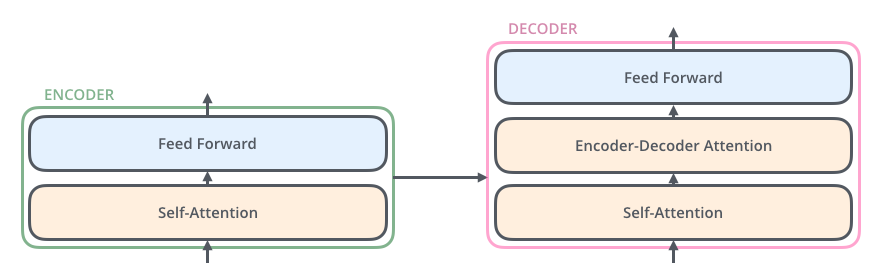
\includegraphics[width=1\columnwidth]{../img/encoder_decoder}
\protect\caption{This picture describes design of one transformers layer. source: http://jalammar.github.io/illustrated-transformer }
\label{pic:enco_deco}
\end{figure}

\begin{figure}[h]
\centering
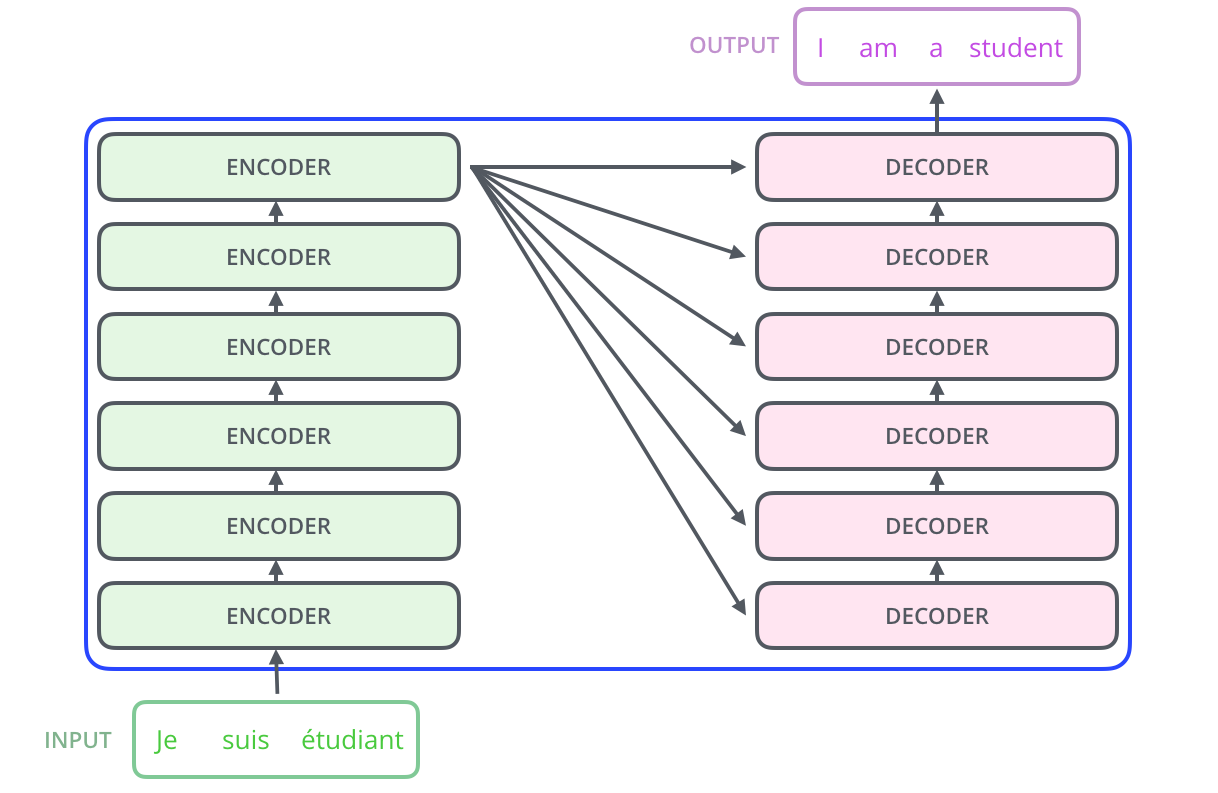
\includegraphics[width=1\columnwidth]{../img/encoder_decoder_all}
\protect\caption{ In transformers, encoder and decoder parts are both composed by many of block of respective types. The input goes first through a series of encoders and than the output of encoder part is put into every decoder in the decoder part. %TODO říct proč 
source: http://jalammar.github.io/illustrated-transformer/  }
\label{pic:enco_deco_all}
\end{figure}

%TODO a  encoder_decoder_all
Self-attention mechanism which is supposed to select most important words to be focused on is used on many places -- for input of every encoder layer, input of every decoder layer (although masked) and also between encoder and decoder. On the decoder side, self-attention layer is masked so the decoder can "see" just previous words (there are $-inf$ values in the positions on the right side). For representation of word position in the sentence (as it is not RNN cell and it can process all words simultaneously) Transformers uses position embeddings, which are trained to represent the ordering in the sentence.
%fixed length vector
%recurrent and shortuct links,normalization


%%%%%%%%%%%%%%%%%%%%%%%%%%%%%%%%%%%%%%%%%%%Relevant methods
\section{BERT explanation}
\label{sec:bert}
This work mainly relies on Bidirectional Encoder Representations from Transformers (BERT) \citep{Devlin2019}, so this section describes and explains main mechanisms of this model. Importance of BERT model is connected with an idea of \textit{transfer learning}. This techniques uses previously learned knowledge and applies such pretrained model on another task \citep{Feijo2020}. BERT is an example of such technique. BERT is trained on two tasks -- next sentence prediction and masked language modelling, but its strength does not lie directly in an ability to predict missing word. These two task are just a way how to teach a model something important about language in general. Final model can be used for almost every NLP task just by changing classification head. There are generaly two ways, how to transfer learned knowledge \citep{Feijo2020}: extract some representation from the model and use in another model statically or modify a model by changing the head and \textit{finetunne} the whole newly created model for specific task. There is also a possibility to combine both approaches and at first take static features as an input for trainig and than, when the head starts to perform well, finetune whole model with this better head, so the original weights converge more efficiently to wanted solution.

%TODO jak je super, že to je bidirectional

%TODO dky se to objevil ten transfer learning, v čem se bert neliší a v čem ano.
The core of BERT algorithm is based on these three features -- two unsupervised task for pretraining, input and its embeddings and transformers encoder architecture. %TODO něco o tom transfer learningu?

\subsection{Input embeddings}
%todo obrazek
BERT uses concatenation of three types of embeddings as an input representation -- token embeddings, position embeddings and segment embeddings. %todo figura z berta

\begin{figure}[h]
\centering
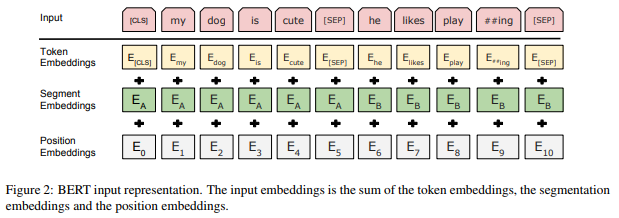
\includegraphics[width=1\columnwidth]{../img/bert_embeddings}
\protect\caption{ Input is representing using tree kinds of embeddings.
Source: \textit{\citep{Devlin2019}}.}
\label{pic:bert_emb}
\end{figure}

\subsubsection*{Token embeddings}
Input of BERT model can be one or two word sequences (not necessarily two sentences, but e.g. also paragraphs). All words are split into tokens and converted into embeddings with a use of pretrained embeddings model. One word can be tokenized into more tokens, because BERT uses WordPiece %todo zdroj
embeddings \citep{Wu2016}. WordPiece pretrained embedding algorithm was originaly created for task of Google voice search for Asian languages and is designed to minimize an occurrence of unknown word tokens. %TODO někam napsat proč se tohle děje
WordPiece model was not pretrained as a part of BERT paper experiments, but represents quite interesting solution, so I will briefly explain the idea. It is impossible to prepare embeddings for every possible word in a language, because this would cause intractably long size of embeddings. Every word which is not a part of selected embedding set is encoded in the same way as a unknown word. This situation is not desired, because we lost informations about words. WordPiece deals this problem in following manner: In the first iteration of training, the model creates embeddings only for basic characters. In every other iteration, some existing model words are concatenated together in the way that cause the highest likelihood of input text. As a result of this method, some words will be embedded as one word and some will be split into more tokens as can be seen on figure. %todo obrazek
\par
There are three other tokens which are added after this step -- CLS, END, SEP. 
CLS token is added at the beginning of the input and is used as first sequence embedding for classification tasks (as sentence analysis). SEP token separates both sequences and END token is appended at the end. Whole input transformation can be seen on figure \ref{pic:bert_emb}.

\subsubsection*{Position embeddings}
All input tokens are processed simultaneously, that is the reason why BERT is often called \textit{undirectional} rather than \textit{bidirectional}. This featrue causes an absence of information about order of tokens. However, nature of the language is sequential, bunch of words without an order has no language meaning and capturing this problem leaded to recurrent neural networks at first. In BERT is no recurrent cell, and this problem is solved by position embeddings. They have same shape as token embeddings (and also as segment embeddings) and they are learned the same way as other embedding layers. Maximum input size in original BERT is 512 so this embedding layer shoulb be able to represent position from 1 to 512. This learning is a difference from original transformers, where position was also encoded as embeddings, but they  were fixed, not learned.

\subsubsection*{Segment embeddings}
These emebddings just indicates whether the token belongs to first or second part of input. It has same dimension as position and token embeddings and they are also learned. Beccause BERT input can consist from at most two parts, segment embeddings just encode whether the token belongs to first or second part.

\subsection{Pretraining tasks}

%TODO narozdil od jinych modelu co jsou trenovane jednosmerne blabla...
BERT is pretrained on two unsupervised tasks -- Next Sentence Prediction (NSP) and Masked LM (MLM). These two tasks were chosen specifically because BERT's authors belief they can force language model to learn general and useful knowledge about language. 

\subsubsection*{Next Sentence Prediction}
Input of the BERT model for this task are two sentences, A and B. In 50\% of cases, sentence B is sentence which really follows sentence A in the source text. Otherwise it is random sentence from the text. A goal of the task is decision whether sentence B is following or random, i.e. binary classification. Motivation for this task is a need to represent relationships between sentences, not only between words. Experiments in \citep{
Devlin2019} showed its usefulness for text tasks as question answering. Sentence-level classification with BERT as in this case can be performed by using last hidden representation of CLS token (first token of every input example). Authors assume that this token can work as a summary of the whole sentence.

\subsubsection*{Masked Language Modeling}
Masked Language Modeling or in other words Cloze task \citep{Taylor1953}
consist of prediction of some missing words in text. In the case of BERT, its implementing in the following way: 15\% of tokens in each sequence are chosen. For each of this chosen tokens there is 80\% chance to be replaced by MASK token, 10\% chance to by replaced by random token or it will remain unchanged with 10\% probability. This ensures that the model will try to predict tokens not only in the case of MASK token presence. For backpropagation, only predictions of MASK token are taken into account. Prediction is done by a softmax function which input is last hidden representation of respective token and softmax layer outputs a probability distribution for prediction of every possible word.

\subsection{Transformers encoder architecture}
BERT adapts encoder part of architecture from original Transformers paper   \citep{Vaswani2017} (see section \ref{sub:transformers}).
Actually, BERT uses its encoder architecture for each layer, 
%todo odkaz a vysvetlit
 o there is L (e.g. 12 in the case of BERT base model) encoder layers finished with one fully connected layer for specific task. In pretraining, there is only one layer responsible for MLM and NSP, as each task uses different part of last hidden layer informations. %todo obrazek architektury
 
 %TODO hyperparametry 
 %TODO dalsi modely - model compression je popsaná v článku Liu2020
 %TODO liu2020 predstavuje co potrebujeme vedet - co by se dalo zkoumat
 %TODO v cem jsou dobre
 \subsection{Why is BERT so special?}
 \label{sub:specialBert}
 %napsat ze je special a proc -- vysledky, asi v teorii a odkaz dát sem
For deep learning architectures, it is quite common that reason why they work (especially why they work so well in comparison with other posibilities) is not visible at first sight. Authors offers following explanation. In contrast to other SOTA league language models, BERT uses both bidirectional context of words. In the figure %todo obrazek z berta
is a comaprison of two other such models - ELMo and GTP %todo zdroje
. GTP is also based on Transformers architecture, but unlike BERT, it uses decoder part of Transformer. 
GTP uses just left context of the word, as a sentence is proceeded sequentially. ELMo uses LSTM %todo odkaz
with both left-to-right and right-to-left training and concatenates results at the end. BERT is proceeding both sides context simultaneously and due to an architecture, in \textit{every layer} every transformer block has potentially information from every other block (and thus from every other word). That is the reason, why BERT is called \textbf{deeply} bidirectional or also non-directional (because there is no right-to-left or left-to-right direction of processing).
\par
Explanation of why and how BERT works are, however, not so simple. There are many papers on how BERT works, what BERT really learns and know, how BERT architecture can be simplyfied and so on. There actually appeared new term "bertology" for this area of research.
 

